\documentclass[12pt]{article}

\usepackage{EngReport}

\graphicspath{{Images/}}
\bibliography{Sources}
\onehalfspacing
\graphicspath{{images/}}
\geometry{letterpaper, portrait, includeheadfoot=true, hmargin=1in, vmargin=1in}

%\fontsize{font size}{vertsize (usually 1.2x)}\selectfont

\begin{document}
\renewcommand{\familydefault}{\rmdefault}

% \begin{titlepage}
%     \begin{center}
%     {\fontsize{30}{48}\selectfont \bfseries Trabajo práctico N° 1} 
%     \\\vspace{20pt}
%     {\LARGE Computación de Alto Rendimiento} \\
%     \vspace{20pt}
%     \textbf{ Garcia Justo}
%     \vspace{8pt}
%     \\ 2023
%     \vspace{8pt}
%     \end{center}
% \end{titlepage}

\begin{titlepage}
    \centering
    {
\includegraphics[width=0.2\textwidth]{Images/fiuner.png}\par}
    \vspace{1cm}
    {\bfseries\LARGE Universidad Nacional de Entre Ríos \par}
    \vspace{1cm}
    {\scshape\Large Facultad de Ingeniería \par}
    \vspace{3cm}
    {\scshape\Huge Trabajo práctico N° 1\par}
    \vspace{0.5cm}
    {\itshape\Large Computación de Alto Rendimiento \par}
    \vfill
    {\Large Autor: \par}
    {\Large Justo Garcia \par}
    \vfill
    {\Large Agosto 2023 \par}
\end{titlepage}
\graphicspath{{Images/}}
\pagestyle{fancy}
\fancyhf{}
\setlength{\headheight}{30pt}
\renewcommand{\headrulewidth}{0.4pt}
\renewcommand{\footrulewidth}{0.4pt}
\lhead{TP 1 \\ CAR }
\rhead{2023 \\ Garcia Justo}
\rfoot{\textbf{\thepage}}
\lfoot{\vspace{20px} 
\includegraphics[scale=0.07]{Images/fotouner.png}}
\renewcommand*\contentsname{Tabla de contenidos}
\tableofcontents
\pagebreak

% % % % % % % % % % % % % % % % % % %
% % % % %  SAMPLE IMAGE   % % % % % %https://www.overleaf.com/project/64eb940f11b4d5805e560df5
% % % % % % % % % % % % % % % % % % %


% \begin{figure}[h]
%     \centering
%     \includegraphics[width=.95\linewidth]{example-image-a}
%     \caption{** Concept Image Caption **}
%     \label{fig:my_label}
% \end{figure}

% % % % % % % % % % % % % % % % % % % %
% % % % %  REPORT CONTENT   % % % % % %
% % % % % % % % % % % % % % % % % % % %

\fontsize{12}{20}\selectfont{

\graphicspath{{Images/}}

\section{Introducción}
En este informe desarrollaré las actividades propuestas para el trabajo práctico número 1 de Computación de Alto Rendimiento. Iré adjuntando los códigos necesarios, sin embargo recomiendo revisar el repositorio de GitHub \cite{repositorio} de este trabajo para obtener una mejor visualización de las soluciones propuestas.

\pagebreak
\graphicspath{{Images/}}

\section{Ejercicio 1}\label{cap:ej1}
\subsection{Consigna}
    Dados dos procesadores $P_0$ y $_1$ el tiempo que tarda en enviarse un mensaje desde $P_0$ hasta $P_1$ es una función de la longitud del mensaje $T_{comm} = T_{comm(n)}$, donde n es el número de bytes en el mensaje. Si aproximamos esta relación por una recta, entonces
    $$T_{comm} = l = \frac{n}{b}$$
    donde \textbf{l} es la “latencia” y \textbf{b} es el “ancho de banda”. Ambos dependen del hardware, software de red (capa de TCP/IP en Linux) y la librería de paso de mensajes usada (MPI). Para determinar el ancho de banda y latencia de la red, escribir un programa en MPI que envíe paquetes de diferente tamaños y realice una regresión lineal con los datos obtenidos. Obtener los parámetros para cualquier par de procesadores en el cluster. Comparar con los valores nominales de la red utilizada (por ejemplo, para Fast Ethernet: \textbf{b} $\approx$ 100Mbit/sec, \textbf{l} = O(100$\mu$ sec)).

\subsection{Resolución}
Adjunto la resolución del ejercicio uno debajo. Sin embargo, recomiendo visualizarlo en el repositorio de GitHub de este trabajo \cite{justog220_practica-car_2023}.

\subsubsection{Implementación con MPI}
\lstinputlisting[language=C++]{codigos/main1.cpp}

\subsubsection{Ejecución en cluster}
Habiendo resuelto la codificación del ejercicio, me conecté al cluster por SSH y envié mi código. Una vez allí, lo compilé y establecí distintos parámetros para correrlo con SLURM (\ref{fig:scriptSLURM}).

\begin{figure}[H]
    \centering
    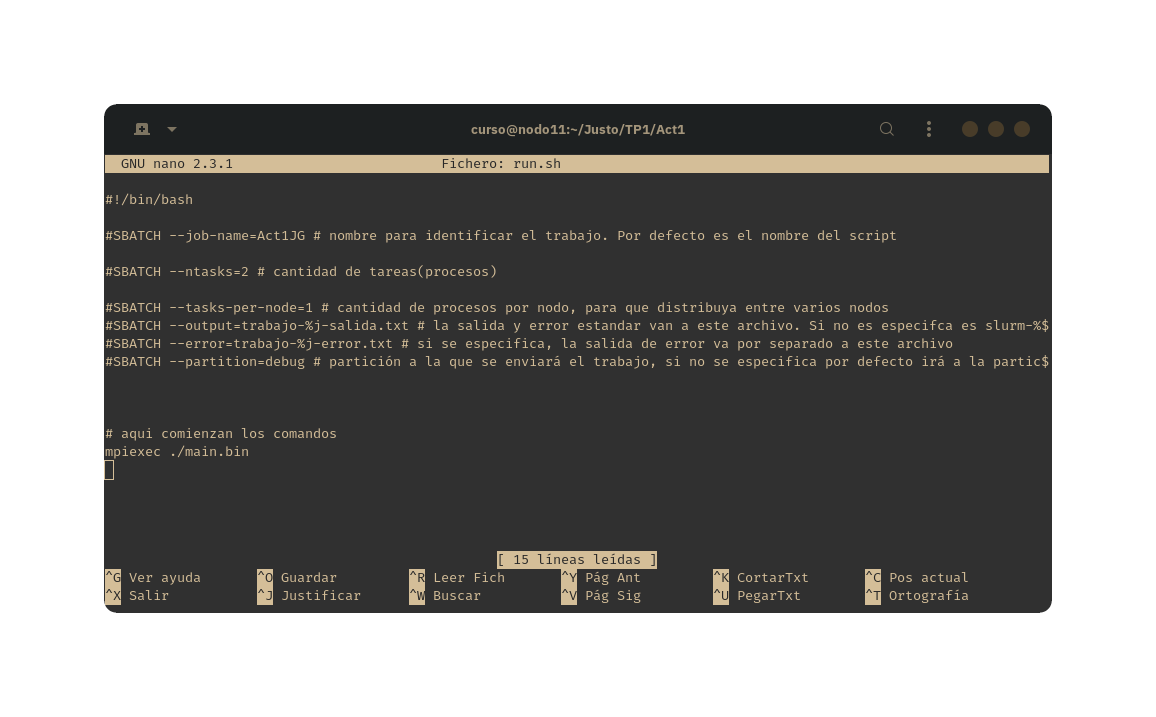
\includegraphics[width=0.60\textwidth]{Images/ej1/Captura desde 2023-08-30 14-22-23.png}
    \caption{Script run.sh para SLURM}
    \label{fig:scriptSLURM}
\end{figure}

Habiendo establecido los parámetros procedo a correrlo con:

\begin{lstlisting}
sbatch run.sh
\end{lstlisting}

Este comando me devuelve el identificador de la tarea lanzada y gestionará su ejecucioón en base a la disponibilidad de cómputo.

Luego observé el estado de mi tarea(\ref{fig:squeue}) con:
\begin{lstlisting}
squeue -l
\end{lstlisting}

\begin{figure}[H]
    \centering
    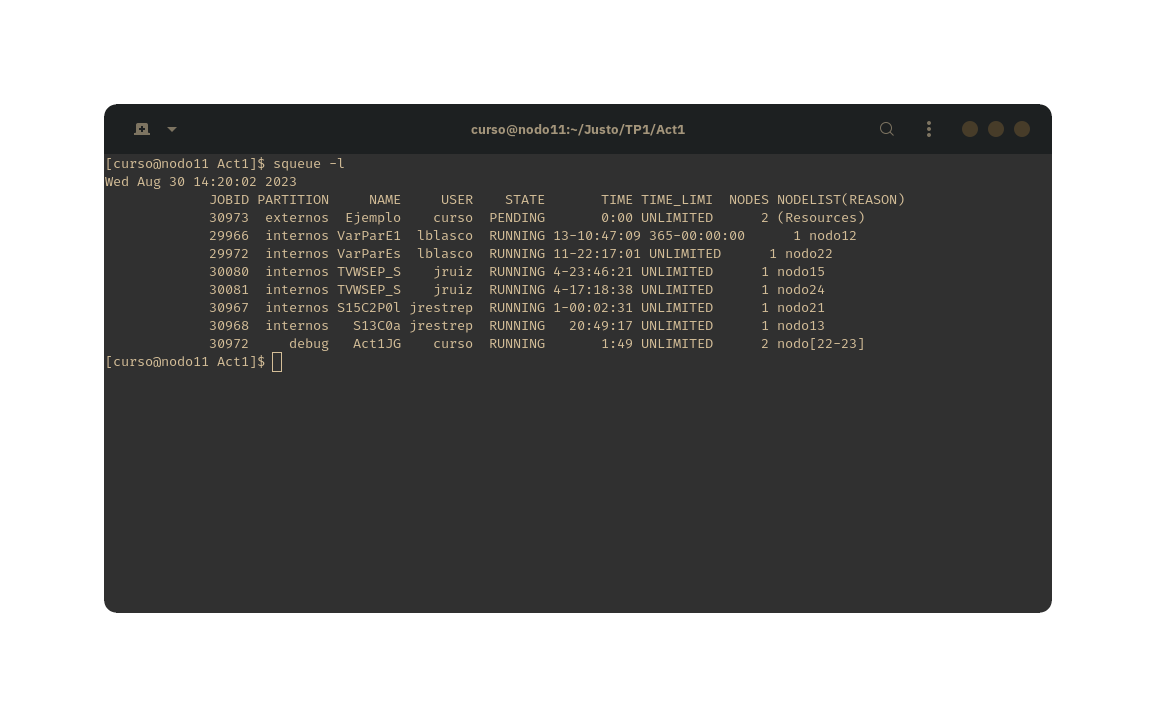
\includegraphics[width=0.60\textwidth]{Images/ej1/Captura desde 2023-08-30 14-20-39.png}
    \caption{Tarea corriendo}
    \label{fig:squeue}
\end{figure}

Finalizada su ejecución, copié la salida en mi dispositivo y realicé el análisis descripto a continuación

\subsubsection{Análisis de resultados}
Habiendo obtenido los datos de latencias realicé un procesamiento de datos con Python, análisis que recomiendo ver en el repositorio de GitHub \cite{justog220_practica-car_2023}.

La salida de mi código fue pensada como valores separados por coma para luego manipularlo facilmente como un archivo de tipo csv. Por ello simplemente hice uso de la librería \textit{pandas} para cargarla como DataFrame y luego analizarla. 

Al momento de la implementación decidí que la medición se realizara 10 veces para poder representar mejor los tiempos para cada tamaño. Por ello tuve que hacer un preprocesamiento para promediarlos. Habiendo realizado esto, obtuve la siguiente tabla:

\begin{table}[H]
\centering
 \begin{tabular}{|c | c|} 
 \hline
    Tamanio & Tiempo \\
    \hline
    1 & 0.000023 \\
    2 & 0.000021 \\
    4 & 0.000021 \\
    8 & 0.000022 \\
    16 & 0.000022 \\
    32 & 0.000022 \\
    64 & 0.000022 \\
    128 & 0.000022 \\
    .. & \\
    8192 & 0.000023 \\
    16384 & 0.000024 \\
    32768 & 0.000027 \\
    65536 & 0.000031 \\
    131072 & 0.000039 \\
    262144 & 0.000054 \\
    524288 & 0.000082 \\
    1048576 & 0.000139 \\
    ... & \\
    1073741824 & 0.120231 \\
 \hline
 \end{tabular}
 \caption{DataFrame obtenido tras la carga de datos}
\label{tab:ej1}
\end{table}

Con los datos ya cargados y promediados hice un análisis exploratorio de los datos con un ScatterPlot \ref{fig:scatterej1}.

\begin{figure}[H]
    \centering
    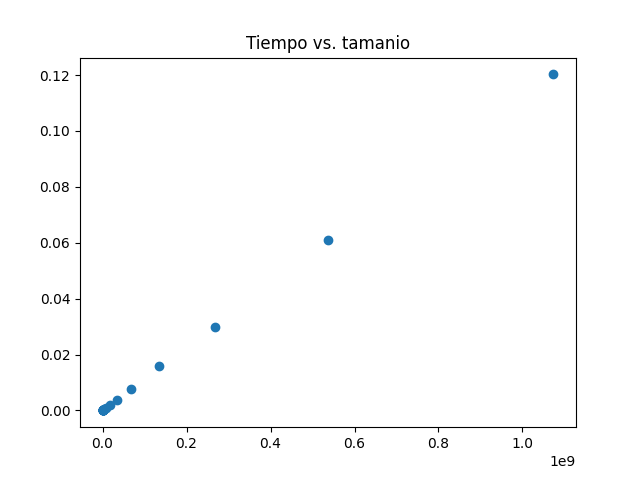
\includegraphics[width=0.60\textwidth]{Images/ej1/scatterej1.png}
    \caption{Scatter plot de los datos}
    \label{fig:scatterej1}
\end{figure}

Se puede observar que los datos parecen tener una relación lineal. Luego, importé de la libreria \textit{SciKit Learn} los módulos necesarios para hacer una regresión lineal con mis datos.

\begin{lstlisting}
    from sklearn.linear_model import LinearRegression

    reg = LinearRegression()

    x = dfProm[["Tamanio"]]
    y = dfProm["Tiempo"]
    
    reg.fit(x, y)
\end{lstlisting}

Teniendo ya la recta que mejor se ajusta a mis datos, la plotee junto al Scatter Plot (\ref{fig:regej1})

\begin{figure}[H]
    \centering
    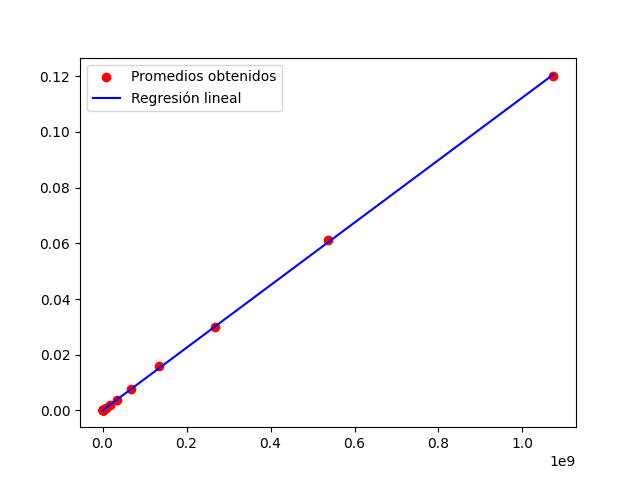
\includegraphics[width=0.60\textwidth]{Images/ej1/reglinej1.png}
    \caption{Datos y la recta ajustada a ellos}
    \label{fig:regej1}
\end{figure}

Habiendo obtenido la regresión lineal, calculé la latencia como la ordenada:

\begin{figure}[H]
    \centering
    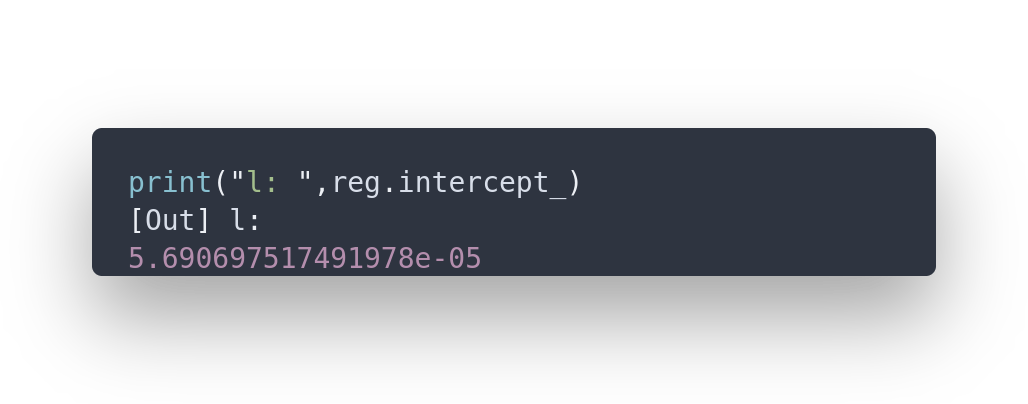
\includegraphics[width=0.60\textwidth]{Images/ej1/intercept.png}
    \caption{Latencia de la red}
    \label{fig:latej1}
\end{figure}

$$l \approx 5,7$$

Luego, de la ecuación de la recta despejé el ancho de banda:
$$b = \frac{n}{T_{comm} - l}$$

Con los datos del DataFrame calculé este dato:
$$b \approx 8905586616.9$$

\pagebreak
\graphicspath{{Images/}}

\section{Ejercicio 2}

\subsection{Consigna}
Para un dado número de procesadores $(n)$ realizar una matriz de transferencia a los fines de detectar posibles heterogeneidades en la velocidad de transferencia de datos entre los procesadores. Analizar la matriz obtenida.

\subsection{Resolución}

\subsubsection{Implementación con MPI}

\lstinputlisting[language=C++]{codigos/main2.cpp}


\subsubsection{Ejecución en cluster}
Tras haber llevado a cabo la implementación del código, lo pase al cluster y lo compile. Habiéndolo compilado pude observar que tenía 4 nodos disponibles para ejecutarlo. Por sugerencia del profesor decidí correrlo de dos maneras:
\begin{enumerate}
  \item Con los 4 nodos y una tarea por nodo.
  \item Con 4 nodos y dos tareas por nodo.
\end{enumerate}

\textbf{Caso 1}

Para correr el primer caso definí el script de SLURM de la siguiente manera:
\begin{figure}[H]
    \centering
    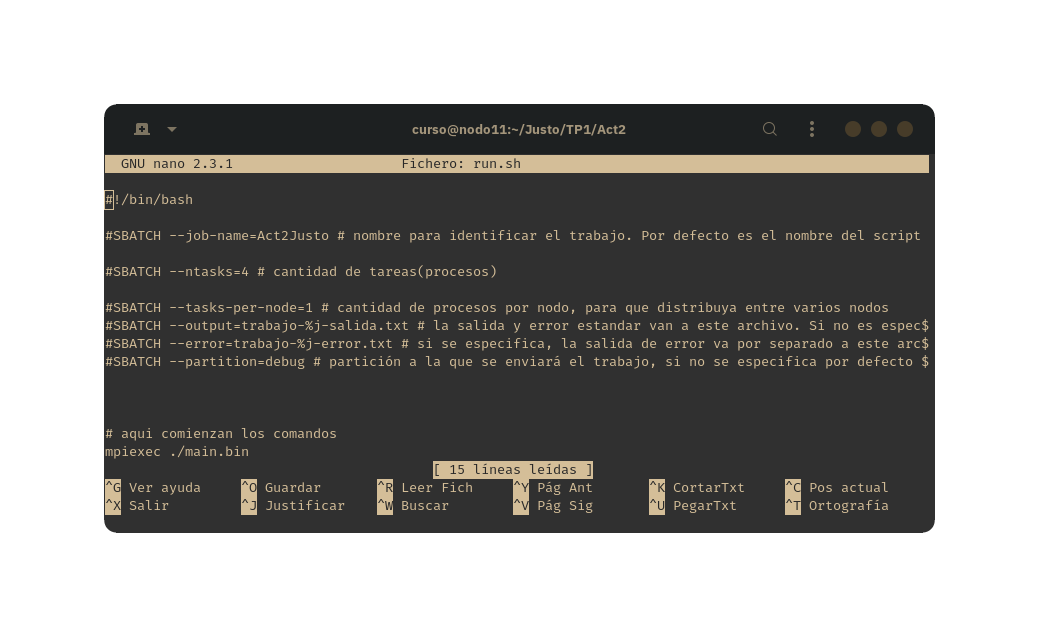
\includegraphics[width=0.80\textwidth]{Images/ej2/scriptcaso1.png}
    \caption{Script para el caso 1}
    \label{fig:scriptcaso1}
\end{figure}

\textbf{Caso 2}
En él el script fue definido de la siguiente manera:
\begin{figure}[H]
    \centering
    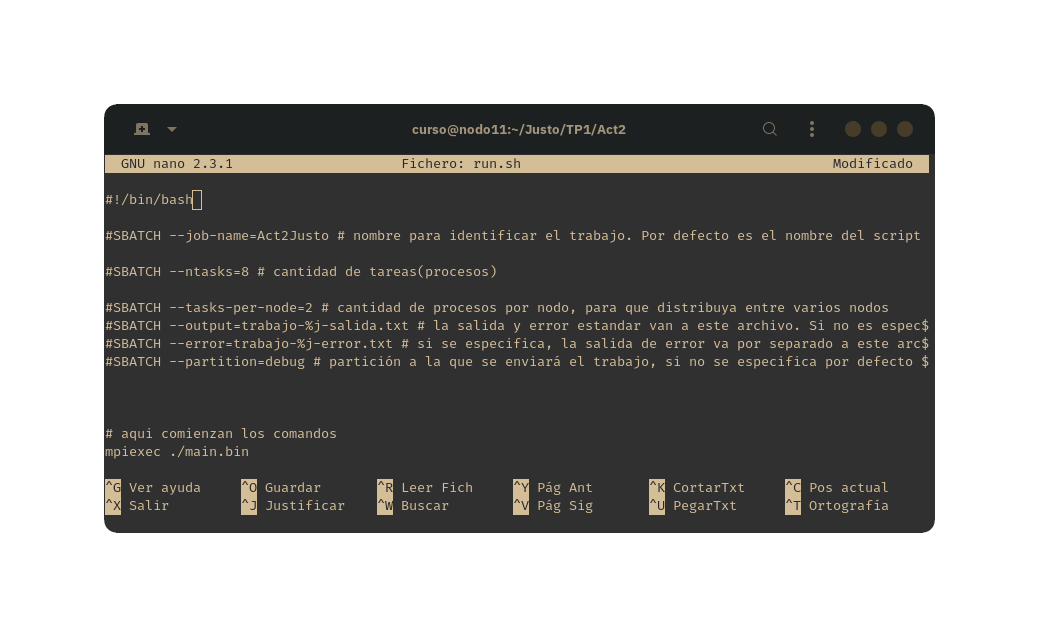
\includegraphics[width=0.80\textwidth]{Images/ej2/scriptcaso2.png}
    \caption{Script para el caso 2}
    \label{fig:scriptcaso2}
\end{figure}

Luego, corrí de igual manera que en el ejercicio 1 (\ref{cap:ej1}) y obtuve las salidas de ambos en mi computadora.


\subsubsection{Análisis}

Teniendo ambos archivos hice un procesamiento de los datos en Python siguiendo la metodología del ejercicio 1 (carga, cálculo del promedio, etc).

Habiendo obtenido un DataFrame para cada caso realicé ciertos cálculos estadísticos, que se ven reflejados en las siguientes tablas: 
\begin{table}[H]
\begin{center}
    \begin{tabular}{| c | c | c | c | }
    \hline
    \multicolumn{2}{|c|}{4 nodos, 1 tarea por nodo} \\ \hline
    Promedio & 0.032750 \\ 
    Desvío & 0.003092 \\ \hline
    \end{tabular}
    \caption{Estadísticos para el caso 1}
    \label{tab:caso1}
\end{center}
\end{table}

\begin{table}[H]
\begin{center}
    \begin{tabular}{| c | c | c | c | }
    \hline
    \multicolumn{2}{|c|}{4 nodos, 2 tareas por nodo} \\ \hline
    Promedio & 0.006535 \\ 
    Desvío & 0.001886 \\ \hline
    \end{tabular}
    \caption{Estadísticos para el caso 2}
    \label{tab:caso2}
\end{center}
\end{table}

Como era de esperarse, el tiempo medio para el caso que tiene más de una tarea por nodo es menor. Esto se debe a que la comunidad entre procesos del mismo nodo es más rápida. 

Luego, realicé mapas de calor para ambos casos de forma que pudiese visualizar gráficamente las diferencias en la latencia.

\textbf{Caso 1}
\begin{figure}[H]
    \centering
    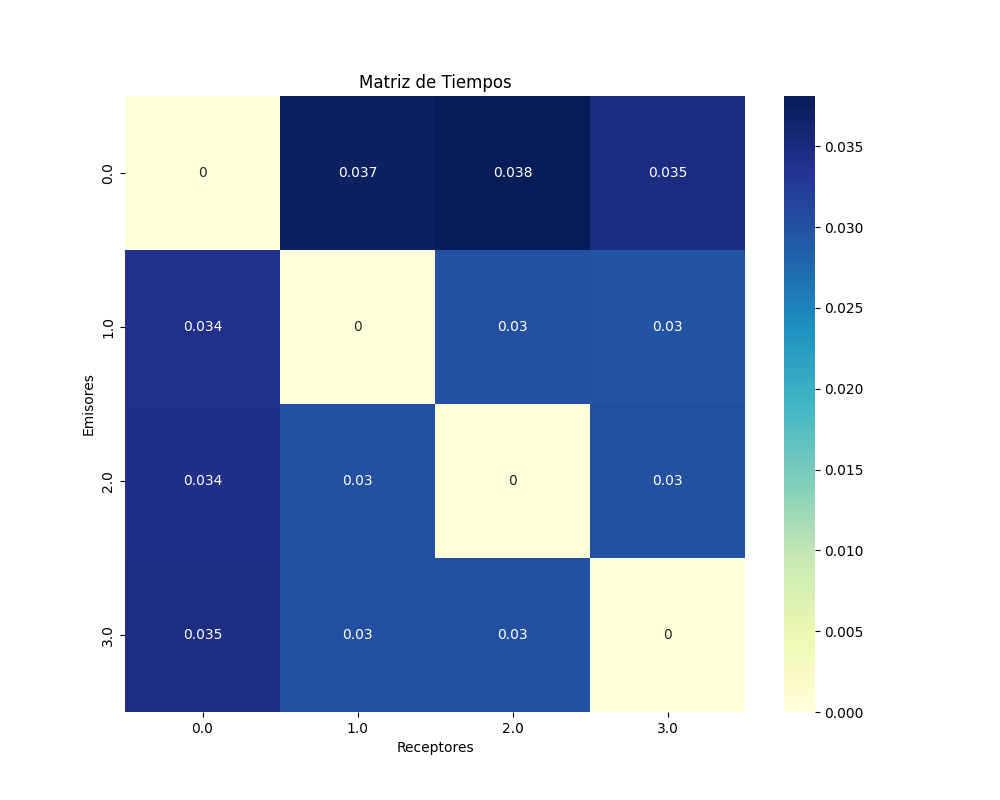
\includegraphics[width=0.80\textwidth]{Images/ej2/matriz1.png}
    \caption{Matriz para el caso 1}
    \label{fig:matrizcaso1}
\end{figure}

Se puede apreciar que cuando tomamos todos nodos distintos, las diferencias son mínimas, y la matriz obtenida es reflejada a través de la diagonal principal.

\textbf{Caso 2}
\begin{figure}[H]
    \centering
    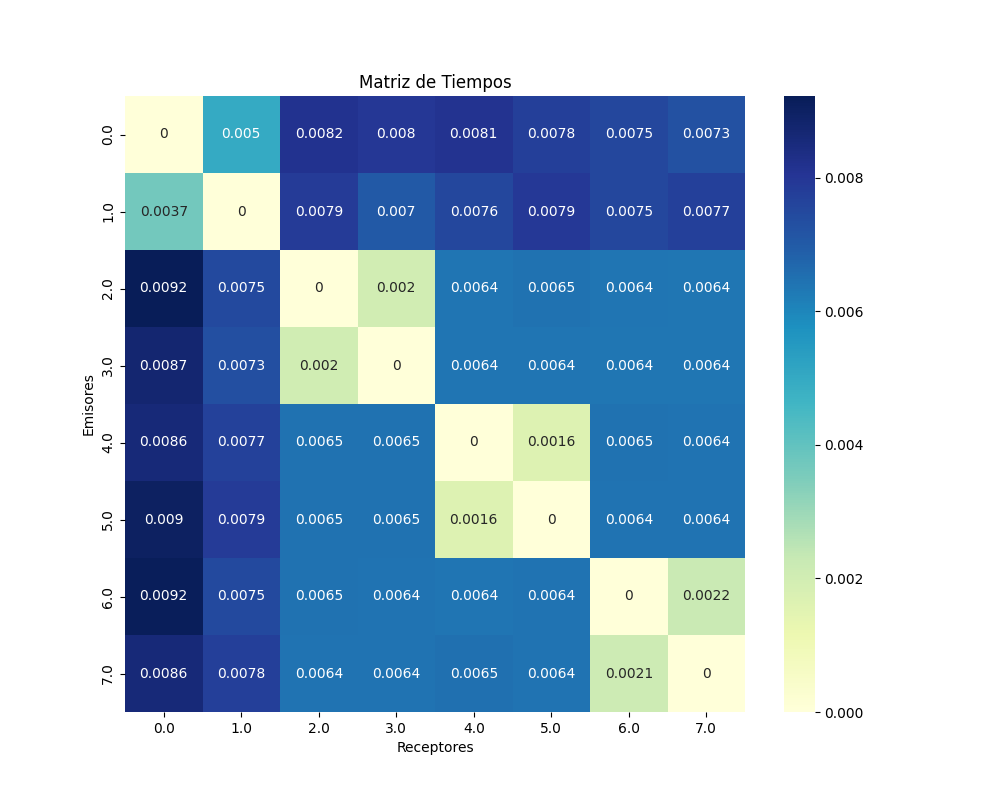
\includegraphics[width=0.80\textwidth]{Images/ej2/matriz2.png}
    \caption{Matriz para el caso 2}
    \label{fig:matrizcaso2}
\end{figure}

En este caso, si vamos tomando de a pares, se pueden ver tiempos muy bajos en comparación con el resto. Esto seguramente se deba a que son procesos que están corriendo en el mismo nodo.
\pagebreak
\graphicspath{{Images/}}

\section{Ejercicio 3}

\subsection{Consigna}
El “ancho de banda de disección” de un cluster es la velocidad con la cual se transfieren datos simultáneamente desde n/2 de los procesadores a los otros n/2 procesadores. Asumiendo que la red es switcheada y que todos los procesadores están conectados al mismo switch, la velocidad de transferencia debería ser $\frac{n}{2}.b$ , pero podría ser que el switch tenga una máxima tasa de transferencia interna


\begin{figure}[h]
    \centering
    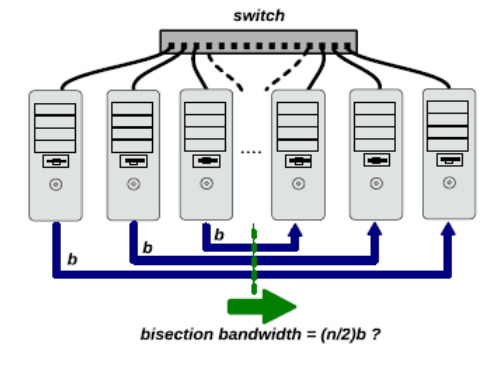
\includegraphics[width=0.40\textwidth]{Images/ej3.png}
\end{figure}

Tomar un número creciente de $n$ procesadores, dividirlos arbitrariamente por la mitad y medir el ancho de banda para esa partición. Comprobar si el ancho de banda de disección crece linealmente con n, es decir si existe algún límite interno para transferencia del switch.

\subsection{Resolución}
\subsubsection{Implementación con MPI}
\lstinputlisting[language=C++]{codigos/main3.cpp}

\subsubsection{Ejecución}
A diferencia de los dos primeros su ejecución se llevó a cabo en uno de los clusters del CIMEC, por lo tanto no se cuenta con ciertos detalles informados en el resto de ejercicios.

\subsubsection{Análisis}
Habiendo finalizado la ejecución obtuve un archivo csv que cargue como DataFrame en python. Como corrí muchas veces el mismo proceso para representar mejor la situación, obtuve el promedio.

Con los datos ya promediados, calculé el ancho de banda de la siguiente forma:

$$b = \frac{\text{Tamaño de paquete}*\text{Nro de procesadores}}{t_{(\text{Nro de procesadores})}}$$

Con estos nuevos cálculos el DataFrame quedó de la siguiente forma: 

\begin{table}[h!]
\centering
 \begin{tabular}{|c |c| c|} 
 \hline
        Nro de procesadores &  Tiempo &  b \\
        \hline
        2.0 &    0.122060 &       5734.875086 \\
        \hline
        4.0 &    0.118834 &       11781.140078 \\
        \hline
        ... &    ... &       ... \\
        \hline
        42.0 &    0.120583 &       121907.428309 \\
        \hline
        44.0 &    0.120362 &        127947.252499 \\
 \hline
 \end{tabular}
 \caption{DataFrame obtenido}
\label{fig:dfej3}
\end{table}

Con estos cálculos ya realizados procedí a graficar tanto el tiempo como el ancho de banda vs. el número de procesadores. (\ref{fig:fig2ej3}, \ref{fig:fig1ej3})

\begin{figure}[H]
    \centering
    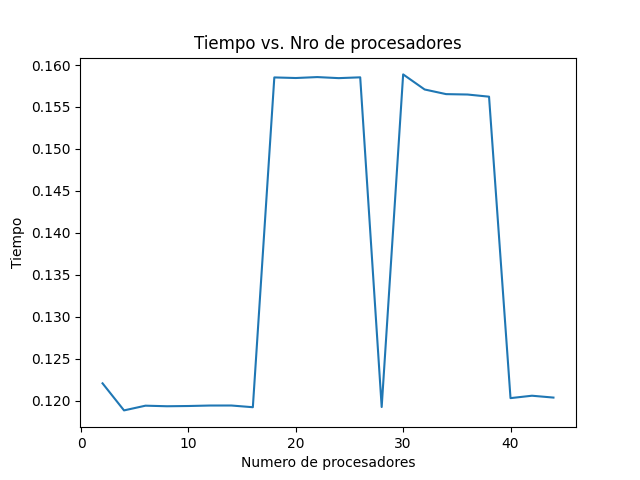
\includegraphics[width=0.60\textwidth]{Images/ej3/fig2ej3.png}
    \caption{Tiempo vs. el número de procesadores}
    \label{fig:fig2ej3}
\end{figure}

\begin{figure}[H]
    \centering
    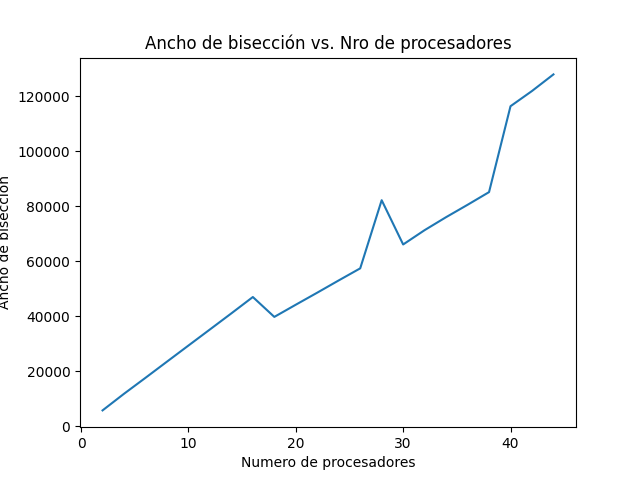
\includegraphics[width=0.60\textwidth]{Images/ej3/fig1ej3.png}
    \caption{Ancho de banda vs. el número de procesadores}
    \label{fig:fig1ej3}
\end{figure}

Como se puede ver observar en la fig \ref{fig:fig2ej3}, el tiempo tiene ciertas irregularidades, pero observando los extremos, podemos ver que no aumenta significativamente. Estas irregularidades pueden deberse a que la configuración de los nodos consta de dos switches distintos. Por otro lado, en la gráfica del ancho de banda no se logra apreciar que se alcance una cota. Este fenómeno se debe a que no se alcanzaron los límites del switch, en caso de disponer de más nodos o enviar un paquete más grande podría alcanzarse. 
\pagebreak
\graphicspath{{Images/}}

\section{Ejercicio 4}

\subsection{Consigna}

Escribir un programa que dado el archivo \emph{homo\_sapiens\_chromosome\_1.fasta}, lo particione en \textbf{n} partes (donde \textbf{n} es el número total del procesadores), envíe cada una de esas porciones a los respectivos procesos y busque la cantidad de veces que aparece la base A (adenina), devolviendo al master la cantidad de veces que cada proceso contabilizó. Finalmente calcule el porcentaje de A en el cromosoma.

\subsection{Resolución}
\subsubsection{Implementación con MPI}

\lstinputlisting[language=C++]{codigos/main4.cpp}


\subsubsection{Ejecución}
Para compilar el código propuesto utilicé el comando:
\begin{lstlisting}
    mpicxx.mpich -o main.bin main.cpp
\end{lstlisting}

Habiendo compilado el código procedí a correrlo con el siguiente comando:

\begin{lstlisting}
    mpiexec.mpich -n n ./main.bin
\end{lstlisting}

\hspace{5mm} Siendo \textit{n} el número de procesos.

Tras finalizada su ejecución, la salida se guarda con formato csv para que luego sea facilmente manipulado con la libreria pandas.

\subsubsection{Análisis}

%insertar análisis%
Habiendo obtenido el número de ocurrencias procedí a cargar los datos a un DataFrame(\ref{fig:dfej4}) de la librería pandas \cite{noauthor_pandasdataframe_nodate}. Allí generé gráficas de barra con el número de ocurrencias para cada una de las bases (\ref{fig:grafica1ej4}). Luego realicé el cálculo de los porcentajes y, de la misma forma que las ocurrencias, las visualicé (\ref{fig:grafica2ej4}).



% \begin{figure}[H]
%     \centering
%     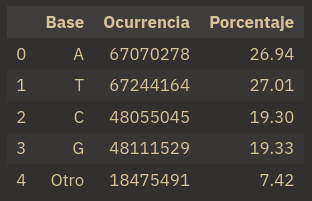
\includegraphics[width=0.35\textwidth]{Images/Captura desde 2023-08-29 18-54-27.png}
%     % \caption{DataFrame obtenido tras la carga de datos}
%     % \label{fig:dfej4}
% \end{figure}


\begin{table}[h!]
\centering
 \begin{tabular}{|c c c|} 
 \hline
        Base &  Ocurrencia &  Porcentaje \\
        \hline
        A &    67070278 &       26.94 \\
        \hline
        T &    67244164 &       27.01 \\
        \hline
        C &    48055045 &       19.30 \\
        \hline
        G &    48111529 &       19.33 \\
        \hline
        Otro &    18475491 &        7.42 \\
 \hline
 \end{tabular}
 \caption{DataFrame obtenido tras la carga de datos}
\label{fig:dfej4}
\end{table}

\begin{figure}[H]
    \centering
    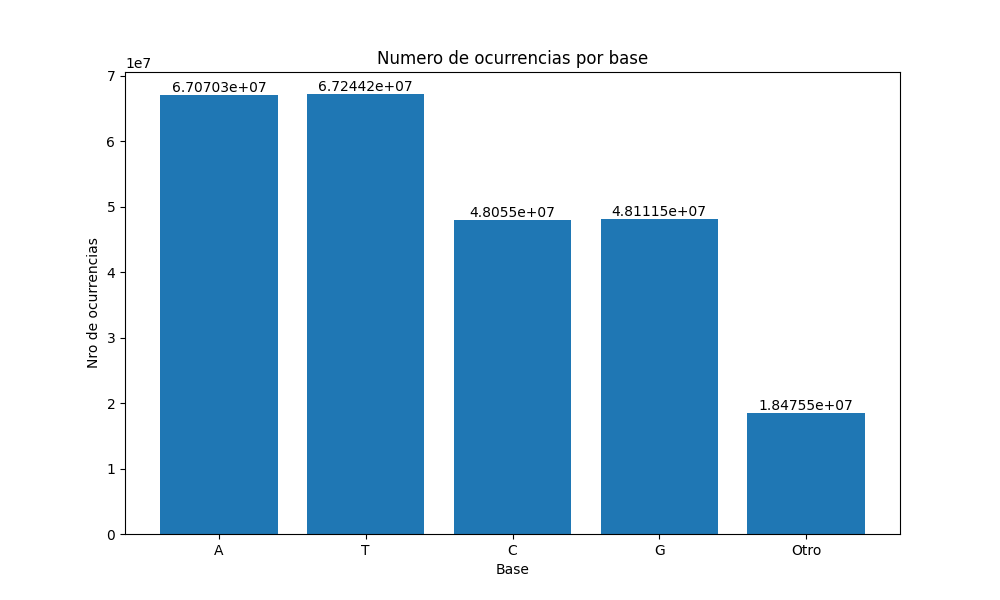
\includegraphics[width=0.70\textwidth]{Images/fig1.png}
    \caption{Gráfico de barra del número de ocurrencia por base}
    \label{fig:grafica1ej4}
\end{figure}

\begin{figure}[H]
    \centering
    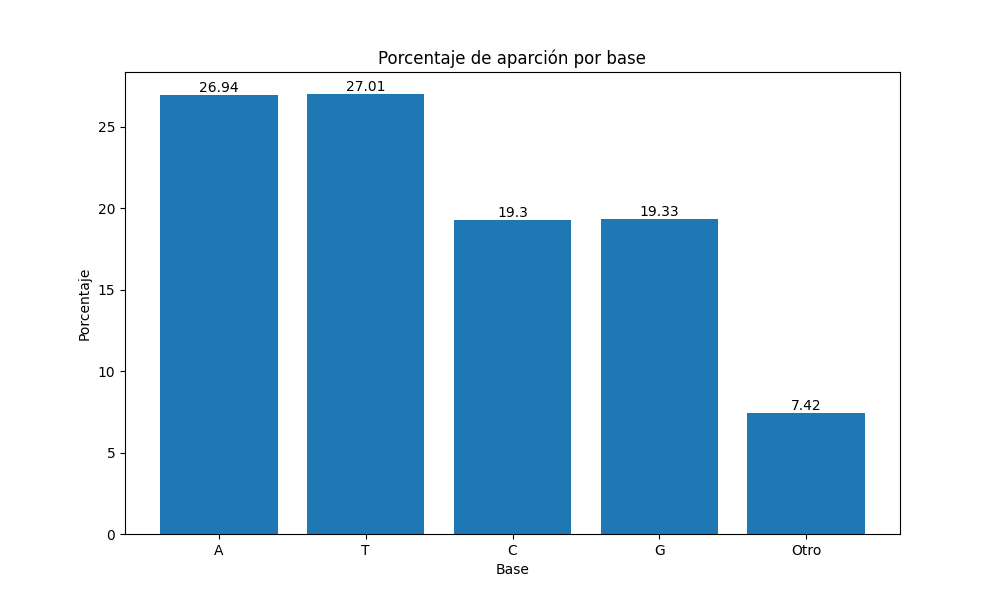
\includegraphics[width=0.70\textwidth]{Images/fig2.png}   
    \caption{Gráfico de barra del porcentaje de aparición de cada base}
    \label{fig:grafica2ej4}
\end{figure}

Por otro lado, decidí comprobar los resultados obtenidos con un script de bash. En él conte el número de ocurrencias con utilidades propias de este interpreté y obtuve los mismos resultados.

%insertar codigo%
El script mencionado es el siguiente:
% \begin{lstlisting}
% #!/bin/bash
% ocurrencias=$(grep -o "A" data/*fasta | wc -l)
% echo "El número de ocurrencias de A es: $ocurrencias"

% ocurrencias=$(grep -o "T" data/*fasta | wc -l)
% echo "El número de ocurrencias de T es: $ocurrencias"

% ocurrencias=$(grep -o "G" data/*fasta | wc -l)
% echo "El número de ocurrencias de G es: $ocurrencias"

% ocurrencias=$(grep -o "C" data/*fasta | wc -l)
% echo "El número de ocurrencias de C es: $ocurrencias"
% \end{lstlisting}

\begin{figure}[H]
    \centering
    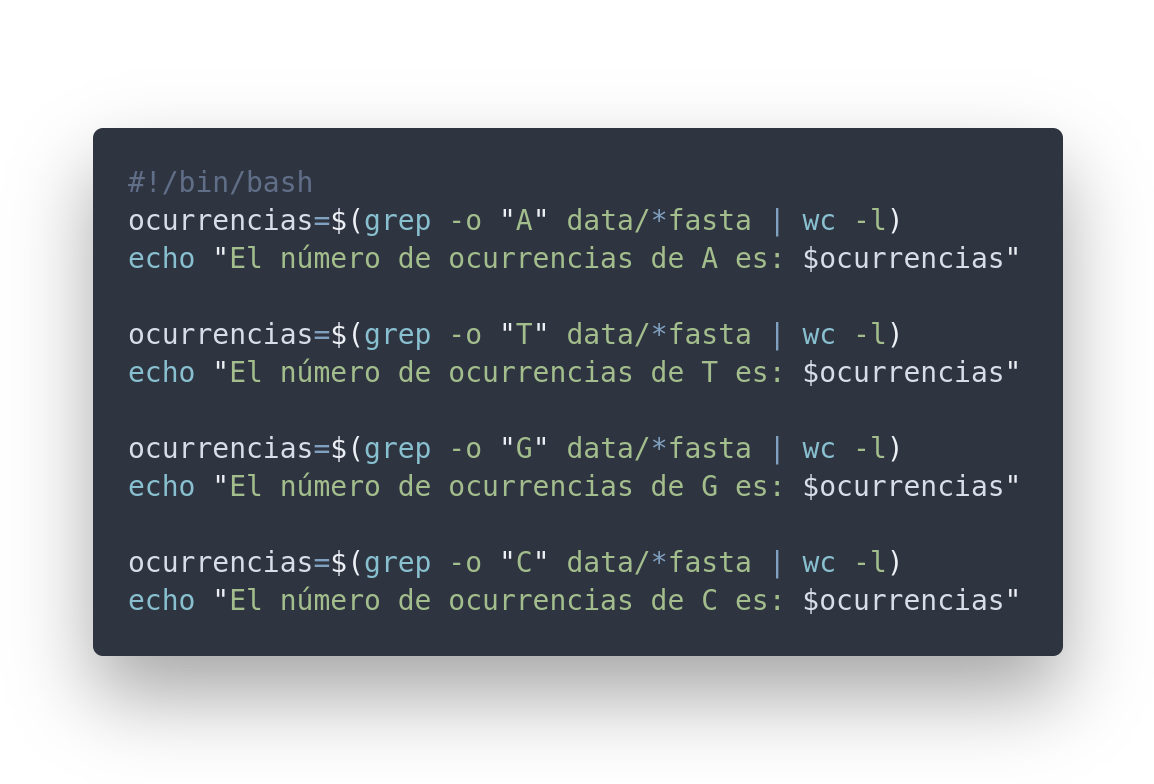
\includegraphics[width=0.70\textwidth]{Images/ej4/script.png}
    \caption{Script implementado}
    \label{fig:scriptej4}
\end{figure}

Tras ejecutarlo, obtuve la siguiente salida (\ref{fig:salidaej4}), que como se puede apreciar, concuerda con los datos obtenidos del procesamiento en paralelo con MPI:



\begin{figure}[H]
    \centering
    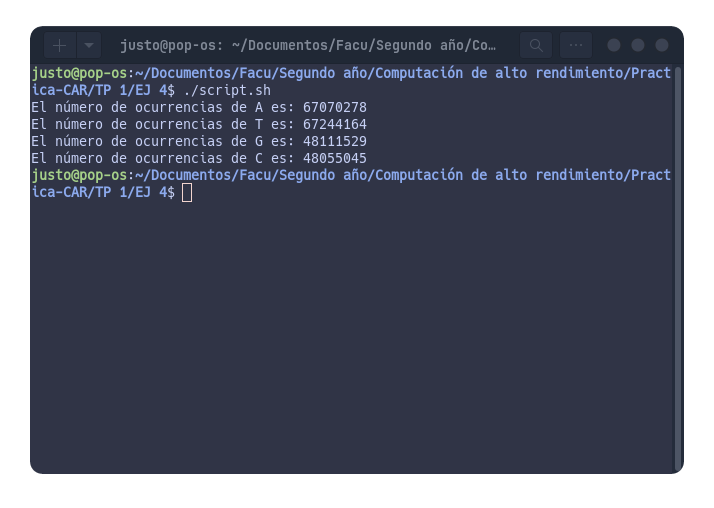
\includegraphics[width=0.80\textwidth]{Images/Captura desde 2023-08-29 16-57-42.png}
    \caption{Salida obtenida de script.sh}
    \label{fig:salidaej4}
\end{figure}


}

\pagebreak

\printbibliography[title={Referencias}]

\end{document}
